\documentclass[10pt]{report}
\usepackage{epsf}
\usepackage{amsmath}
\usepackage{amssymb}
\usepackage{palatino}
\usepackage[pdftex]{graphics}
\usepackage{fancyhdr}
\usepackage{epsfig}
\usepackage{multirow}
\usepackage{multicol}
\usepackage{cancel}
\usepackage{hyperref}
\usepackage{longtable}
\usepackage{ulem}
\usepackage[yyyymmdd]{datetime}
\renewcommand{\dateseparator}{-}
%\usepackage{draftwatermark}
\usepackage{listings}

\parindent 0in
\parskip 1ex
\oddsidemargin  0in
\evensidemargin 0in
\textheight 8.5in
\textwidth 6.5in
\topmargin -0.25in

\pagestyle{fancy}
\lhead{\textbf{\leftheader}}
\rhead{\textbf{\rightheader}}
\lfoot{Compiled: \today\ \currenttime}
\cfoot{}
\rfoot{\thepage}

\newcommand{\leftheader}{BME290L: MedTech Prototyping Skills}
\newcommand{\rightheader}{Palmeri (Spring 2023)}

\begin{document}
\section*{Lab 01: Software Installation}

\subsection*{Installation}
Please install the following programs on your laptop:
\begin{itemize}
    \item \href{https://kicad.org/}{KiCad} - \texttt{v6.0.10}
    \item \href{https://git-scm.com/}{Git} - version control software
    \item One of the following for firmware development:
    \begin{itemize}
        \item \href{https://code.visualstudio.com/}{Visual Studio Code} with \href{https://platformio.org/}{PlatformIO} extension
        \item \href{https://www.arduino.cc/en/software}{Arduino IDE}
    \end{itemize}
\end{itemize}

\subsection*{Account Login}
Please make sure you can log into each of the following cloud services:
\begin{itemize}
    \item \href{https://gitlab.oit.duke.edu}{GitLab} - version control / project mangement (use Shibboleth)
    \item \href{https://duke.onshape.com}{Onshape} - make sure you use the Duke domain!!
    \item \href{https://teams.microsoft.com}{Teams} - install clients on your devices
\end{itemize}

\subsection*{Test Installations}

\subsubsection*{KiCad}
\begin{itemize}
    \item Download the following zip archive:
    \url{https://gitlab.oit.duke.edu/mlp6/kicad_test/-/archive/main/kicad_test-main.zip}
    \item Launch KiCad, and load the Project.\\
    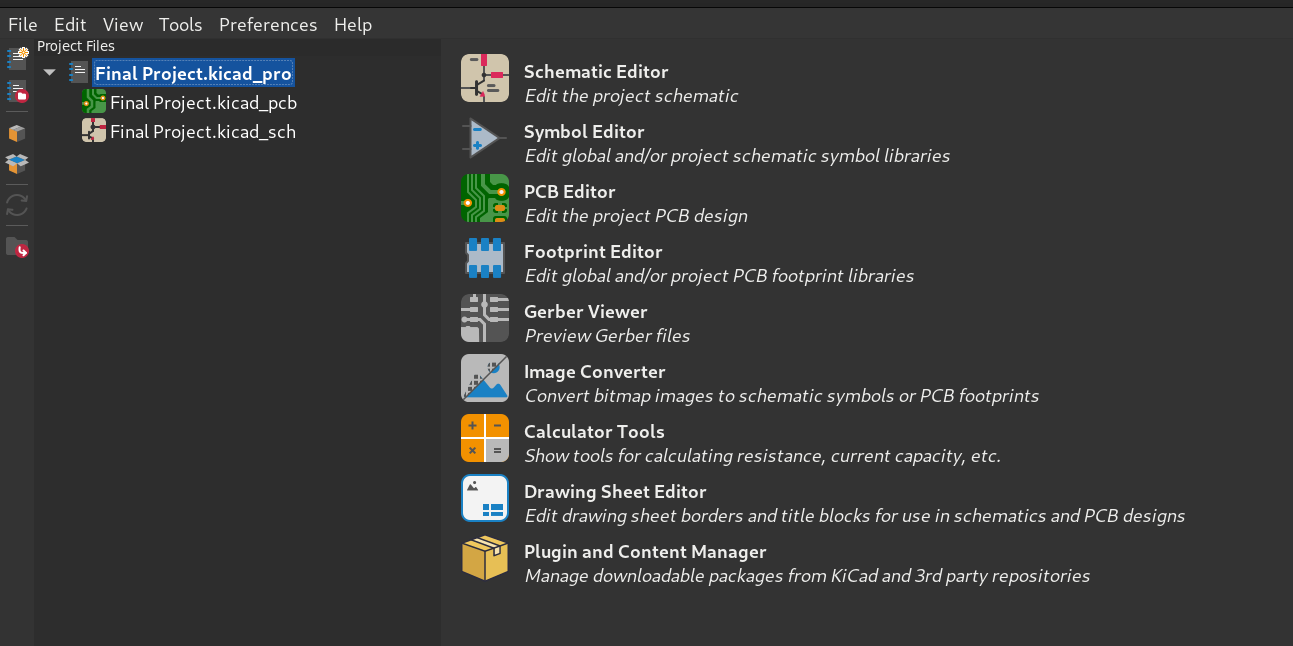
\includegraphics[width=1.0\textwidth]{kicad_screen.png}
    \item Once the project is loaded, confirm that you can open the:
    \begin{itemize}
        \item Schematic (select \texttt{Default} option for library)
        \item PCB (select \texttt{Default} option for library)
        \item Render \texttt{View -> 3D Viewer}
    \end{itemize}
    \item You should see what was shown in lecture for the schematic  and PCB;
    the 3D view will be missing some parts.
\end{itemize}

\subsubsection*{Arduino}
If you don't have one of these following boards, please order one ASAP!
\begin{itemize}
    \item \href{https://store-usa.arduino.cc/products/arduino-nano-33-ble?selectedStore=us}{Arduino Nano 33 BLE} 
    \item \href{https://store-usa.arduino.cc/products/arduino-nano-33-ble-sense?selectedStore=us}{Arduino Nano 33 Sense}
    \item \href{https://store-usa.arduino.cc/products/arduino-nano-every-with-headers?selectedStore=us}{Arduino
    Nano Every}\footnote{This board is being used in BME354L this semester.}
\end{itemize}

When you have your board, run the following test Arduino code and confirm that
you can see the \texttt{Hello World!} messages coming through the serial monitor / TTY device:
\begin{lstlisting}[language=C]
    void setup() {
        Serial.begin(9600);
     }
     void loop() {
        Serial.println("Hello World!");
        delay(1000);
     }
\end{lstlisting}

\end{document}
